\documentclass[../main.tex]{subfiles}

\begin{document}
\section{总体设计}

% 说明,包括:
% 1)数据结构设计
% 2)总体结构设计:包括
% 功能模块的划分
% 模块功能
% 模块之间的关系
% 模块之间的接口
% 3)用户接口设计

\subsection{数据流图}

\begin{figure}[h]
    \centering
    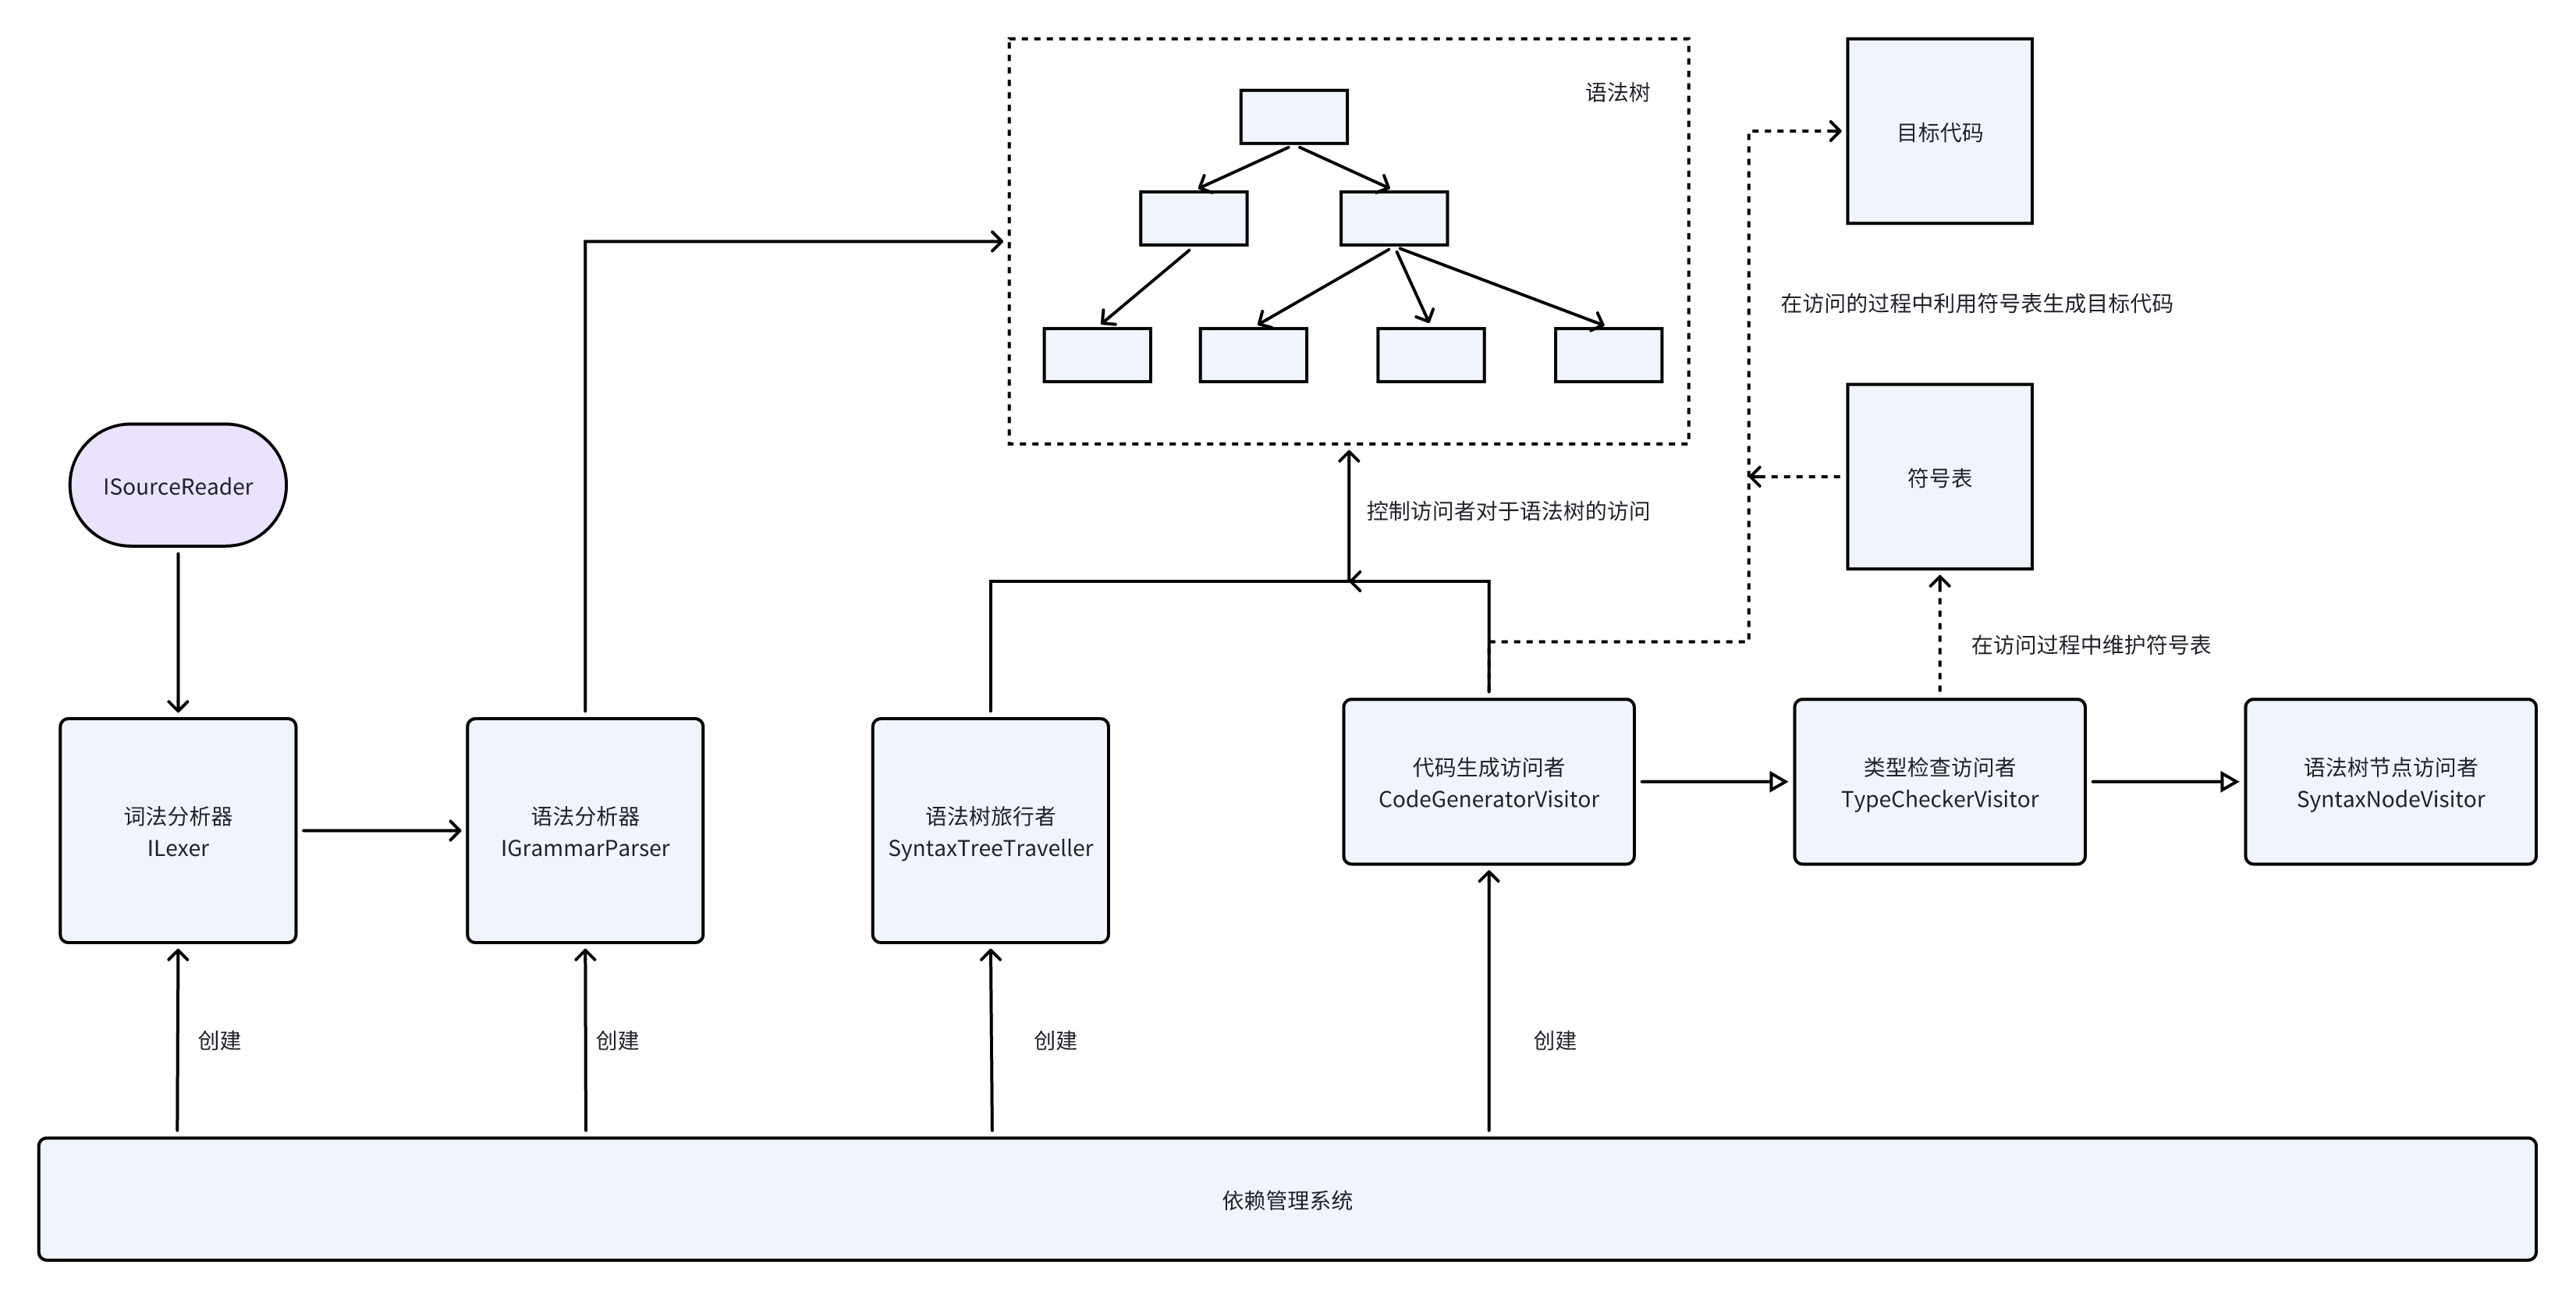
\includegraphics[width=0.9\linewidth]{assets/数据流图.png}
    \caption{数据流图}
    \label{fig:data_flow_diagram}
\end{figure}

\subsection{数据结构设计}

在整个编译器设计中,数据结构的设计是至关重要的一环。它不仅需要支持编译器的各个阶段,还需要保证数据的正确传递和高效处理。在本节中将对编译器中各个模块之间共有的部分数据结构进行说明。

\subsubsection{词法记号}

\texttt{SemanticToken} 是一个抽象基类,定义了所有词法记号的共有属性和方法。具体类型的词法记号(如关键字、标识符等)都继承自这个类。

每个Token至少有四个属性:记号类型 \texttt{SemanticTokenType TokenType},行号 \texttt{uint LinePos},字符位置 \texttt{uint CharacterPos},字面量 \texttt{string LiteralValue}。

\begin{lstlisting}[
    style=csharp
]
public abstract class SemanticToken
{
    public abstract SemanticTokenType TokenType { get; }
    
    /// <summary>
    /// 记号出现的行号
    /// </summary>
    public required uint LinePos { get; init; }
    
    /// <summary>
    /// 记号出现的列号
    /// </summary>
    public required uint CharacterPos { get; init; }
    
    /// <summary>
    /// 记号的字面值
    /// </summary>
    public required string LiteralValue { get; init; }
}
\end{lstlisting}

实际继承词法记号基类的词法记号类有:
\begin{itemize}
\item 字符类型记号 \texttt{CharacterSemanticToken}
\item 字符串类型记号 \texttt{StringSemanticToken}
\item 分隔符类型记号 \texttt{DelimiterSemanticToken}
\item 关键词类型记号 \texttt{KeywordSemanticToken}
\item 操作符类型记号 \texttt{OperatorSemanticToken}
\item 数值类型记号 \texttt{NumberSemanticToken}
\item 标识符类型记号 \texttt{IdentifierSemanticToken}
\end{itemize}

其中分隔符类型、关键词类型、操作符类型等记号提供一个属性获得该记号代表的分隔符、关键词、操作符,这些可以穷举的类型使用枚举标识,在表\ref{table:operator_and_delimiter}和表\ref{table:keyword_and_operator}中列举了所有的分隔符、关键词和操作符。而对于字符类型记号,字符串类型记号、数组类型记号,在代码中分别提供了将字面值识别为C\#中的字符、字符串和数值等类型的功能,方便在代码中对于这种固定值进行操作。在标识符类型中则是提供了一个返回标识符值的方法,在该方法中会自动将字面值小写,以此来提供Pascal代码中对于大小写不敏感的功能。

% \begin{table}[h]
% \centering
% \caption{基本类型和标识符}
% \begin{tabular}{|c|c|c|c|}
% \hline
% \textbf{描述} & \textbf{字面量记录} & \textbf{记号类型} & \textbf{详细类型} \\
% \hline
% 标识符 & 该标识符本身 & IDENTIFIER & \\
% 无符号整数 & 该整数本身(字符串表示) & NUMBER & 整数 \\
% 无符号浮点数 & 该浮点数本身(字符串表示) &  & 实数 \\
% 十六进制数 & 该十六进制数本身(字符串表示) &  & 十六进制 \\
% 字符常量 & 该字符常量本身(不包含两侧的单引号) & CHARACTER & \\
% \hline
% \end{tabular}
% \end{table}

\begin{longtable}{|c|c|c|c|}
\caption{运算符和分界符} \label{table:operator_and_delimiter} \\
\hline
% 跨页表的第一行
\textbf{描述} & \textbf{字面量记录} & \textbf{记号类型} & \textbf{详细类型} \\
\hline
\endhead
% 跨页表的最后一行
\hline
\multicolumn{4}{r@{}}{接下一页}
\endfoot
% 跨页表的最后一页的最后一行
\hline
\endlastfoot
关系运算符 & $\geq$ & Operator & 大于等于 \\
 & $>$ &  & 大于 \\
 & $\leq$ &  & 小于等于 \\
 & $\neq$ &  & 不等于 \\
 & $<$ &  & 小于 \\
关系运算符:相等 & $=$ &  & 等于 \\
算术运算符:加法 & $+$ &  & 加 \\
算术运算符:减法 & $-$ &  & 减 \\
算术运算符:乘法 & $*$ &  & 乘 \\
算术运算符:除法 & $/$ &  & 除 \\
赋值符号 & $:=$ &  & 赋值 \\
范围连接符 & $..$ & Delimiter & 点点 \\
界符 & $($ &  & 左括号 \\
 & $)$ &  & 右括号 \\
 & $[$ &  & 左方括号 \\
 & $]$ &  & 右方括号 \\
 & $:$ &  & 冒号 \\
 & $,$ &  & 逗号 \\
 & $;$ &  & 分号 \\
 & $.$ &  & 句号/点 \\
\hline
\end{longtable}

\begin{longtable}{|c|c|c|c|}
\caption{关键字和逻辑运算符} \label{table:keyword_and_operator} \\
\hline
\textbf{描述} & \textbf{字面量记录} & \textbf{记号类型} & \textbf{详细类型} \\
\hline
\endhead
% 跨页表的最后一行
\hline
\multicolumn{4}{r@{}}{接下一页}
\endfoot
% 跨页表的最后一页的最后一行
\hline
\endlastfoot
逻辑运算符:或 & or & Keyword & 或 \\
算术运算符:取余 & mod &  & 取余 \\
逻辑运算符:且 & and &  & 且 \\
逻辑运算符:非 & not &  & 非 \\
关键字 & program &  & 程序 \\
关键字 & const &  & 常量 \\
关键字 & var &  & 变量 \\
关键字 & array &  & 数组 \\
关键字 & of &  & 属于 \\
关键字 & procedure &  & 过程 \\
关键字 & function &  & 函数 \\
关键字 & begin &  & 开始 \\
关键字 & end &  & 结束 \\
关键字 & if &  & 如果 \\
关键字 & then &  & 那么 \\
关键字 & for &  & 对于 \\
关键字 & to &  & 至 \\
关键字 & do &  & 执行 \\
关键字 & else &  & 否则 \\
关键字 & repeat &  & 重复 \\
关键字 & until &  & 直到 \\
关键字 & while &  & 当 \\
关键字 & integer &  & 整数 \\
关键字 & real &  & 实数 \\
关键字 & char &  & 字符 \\
关键字 & boolean &  & 布尔 \\
\end{longtable}

\subsubsection{语法树}

语法树是编译器中用于表示源代码结构的树状数据结构。在语法分析阶段,编译器将源代码转换为语法树,以便后续阶段可以更高效地进行处理。因此,语法树中每个节点和语法中的每个符号一一对应,其中非终结符即对应书上的父节点,终结符对应了树上的叶子节点。

在终结节点上直接封装了访问对应的词法分析令牌的功能。

\begin{lstlisting}[style=csharp]
public class TerminatedSyntaxNode : SyntaxNodeBase
{
    public override bool IsTerminated => true;

    public required SemanticToken Token { get; init; }

    // 其他代码有删节
}
\end{lstlisting}

在针对不同的非终结节点,首先在其的共同基类\texttt{NonTerminatedSyntaxNode}中封装了访问其子节点的功能,并针对该节点产生式的不同提供了不同的方式模型。

针对只有一个产生式的非终结节点,直接在该非终结节点上使用属性的方式将其有意义的子节点暴露出来,例如在\texttt{ProgramStruct}上就直接暴露放访问\texttt{ProgramHead}的属性。

\begin{lstlisting}[style=csharp]
public class ProgramStruct : NonTerminatedSyntaxNode
{
    public override NonTerminatorType Type => NonTerminatorType.ProgramStruct;

    /// <summary>
    /// 程序头
    /// </summary>
    public ProgramHead Head => Children[0].Convert<ProgramHead>();
}
\end{lstlisting}

针对含有多个产生式的非终结节点,如果是有效的子节点只有一种的,则仍然使用属性的方式进行暴露,例如\texttt{ConstDeclaration},其就暴露了标识符名称和值两个属性。

\begin{lstlisting}[style=csharp]
public class ConstDeclaration : NonTerminatedSyntaxNode
{
    public override NonTerminatorType Type => NonTerminatorType.ConstDeclaration;

    /// <summary>
    /// 是否递归的声明下一个ConstDeclaration
    /// </summary>
    public bool IsRecursive { get; private init; }

    /// <summary>
    /// 获得声明的常量
    /// </summary>
    public (IdentifierSemanticToken, ConstValue) ConstValue => GetConstValue();

    public static ConstDeclaration Create(List<SyntaxNodeBase> children)
    {
        bool isRecursive;
        if (children.Count == 3)
        {
            isRecursive = false;
        }
        else if (children.Count == 5)
        {
            isRecursive = true;
        }
        else
        {
            throw new InvalidOperationException();
        }

        return new ConstDeclaration { Children = children, IsRecursive = isRecursive };
    }

    private static IdentifierSemanticToken ConvertToIdentifierSemanticToken(SyntaxNodeBase node)
    {
        return (IdentifierSemanticToken)node.Convert<TerminatedSyntaxNode>().Token;
    }

    private (IdentifierSemanticToken, ConstValue) GetConstValue()
    {
        if (IsRecursive)
        {
            return (ConvertToIdentifierSemanticToken(Children[2]), Children[4].Convert<ConstValue>());
        }
        else
        {
            return (ConvertToIdentifierSemanticToken(Children[0]), Children[2].Convert<ConstValue>());
        }
    }
}
\end{lstlisting}

而对于使用的多个产生式且无法有效提取信息的非终结节点,则设计使用\textbf{事件}以提供相关信息的功能。访问者可以在需要使用对应产生式的信息时订阅对应的事件,并且语法树的实现保证对应的事件会在第一次访问和第二次访问时按照订阅的顺序进行调用。对应事件的事件参数也可提供产生式相关的信息。

\texttt{ConstValue}就是一个不错的例子,其提供了使用数值产生式和字符产生式的两个事件供订阅。

\begin{lstlisting}[style=csharp]
/// <summary>
/// 使用数值产生式事件的事件参数
/// </summary>
public class NumberConstValueEventArgs : EventArgs
{
    /// <summary>
    /// 是否含有负号
    /// </summary>
    public bool IsNegative { get; init; }

    /// <summary>
    /// 数值记号
    /// </summary>
    public required NumberSemanticToken Token { get; init; }
}

/// <summary>
/// 使用字符产生式事件的事件参数
/// </summary>
public class CharacterConstValueEventArgs : EventArgs
{
    /// <summary>
    /// 字符记号
    /// </summary>
    public required CharacterSemanticToken Token { get; init; }
}

public class ConstValue : NonTerminatedSyntaxNode
{
    public override NonTerminatorType Type => NonTerminatorType.ConstValue;

    /// <summary>
    /// 使用数值产生式的事件
    /// </summary>
    public event EventHandler<NumberConstValueEventArgs>? OnNumberGenerator;

    /// <summary>
    /// 使用字符产生式的事件
    /// </summary>
    public event EventHandler<CharacterConstValueEventArgs>? OnCharacterGenerator;
}
\end{lstlisting}

\subsubsection{符号表}

符号表是在语义分析阶段使用的数据结构,用于存储变量、函数和过程的信息。符号表支持查询、插入和作用域管理操作。每个作用域都有自己的符号表,如果当前作用域中没有找到符号,则会递归查询父作用域。

符号表的设计如下:

\begin{itemize}
    \item \textbf{符号表项(SymbolTableItem)}:包含类型(MegaType)、名称、是否为变量、是否为函数和参数列表。
    \item \textbf{类型(MegaType)}:包含指针类型和项类型。
\end{itemize}

符号表的物理结构采用哈希表实现,以支持高效的查询和插入操作。

\subsubsection{语法树上的旅行者}

在语法分析完成对于语法树的构建之后,我们需要在语法树的各个节点上进行一系列的操作,例如进行符号表的维护、类型检查和代码生成等任务。为了降低程序的复杂度,我们希望在程序中提供一个统一的语法树遍历和访问接口。因此,我们使用访问者设计模式设计了\texttt{SyntaxNodeVisitor}(语法节点访问者)和\texttt{SyntaxTreeTraveller}(语法树旅行者)。同时结合编译原理课程中语义分析和翻译方案相关的知识,我们设计了一种称为\textit{前后序遍历}的语法树访问模型。例如对于图\ref{fig:syntax_tree_example}中的一颗语法树,其的遍历顺序为

\begin{align}\notag
& ProgramStruct \to ProgramHead \to program \to program \to main \to main \\ \notag
&\to ProgramHead \to ; \to ; \to ProgramBody \to ConstDeclarations \to \\ \notag
&ConstDelcarations \to VarDeclarations \to VarDeclarations \to \\ \notag
&SubprogramDeclarations \to SubprogramDeclarations \to CompoundStatement \\ \notag
&\to begin \to begin \to StatementList \to Statement \to Statement \to \\ \notag
&StatementList \to end \to end \to CompoundStatement \to ProgramBody \\ \notag
&\to . \to . \to ProgramStruct \notag
\end{align}

\begin{figure}[t]
    \centering
    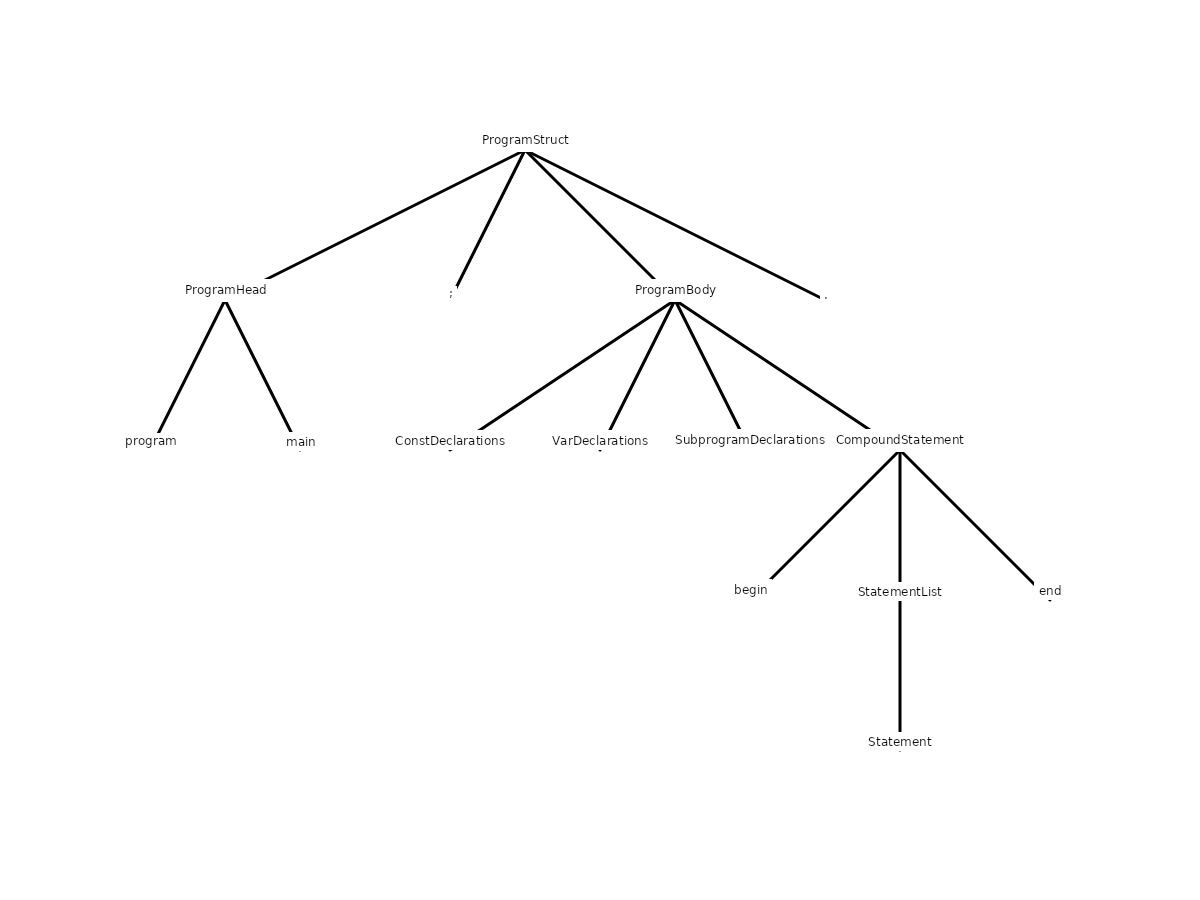
\includegraphics[width=0.9\linewidth]{assets/示例语法树图.png}
    \caption{示例的语法树图}
    \label{fig:syntax_tree_example}
\end{figure}

在设计对于语法树的遍历之后,我们在设计了对于语法节点的访问者,访问者针对语法树上的每一个节点都提供了两个访问接口,分别会在第一次遍历到该节点和第二次遍历到该节点时调用,称为\texttt{PreVisit}和\texttt{PostVisit}。按照编译原理课程中的知识来说,\texttt{PreVisit}接口理解为对于该节点的L-属性计算,\texttt{PostVisit}接口理解为对该节点的S-属性计算。

为了使得各语义分析的工作可以方便的组合在一起运行,例如类型检查需要在代码检查之前运行,容易想到使用类型继承的方式进行抽象。例如类型检查类直接继承了语法节点访问者抽象基类\texttt{SyntaxNodeVisitor},而代码生成了则直接继承了类型检查类。需要注意的是,在重载访问语法节点的接口函数之间,需要在执行任何操作之前调用基类的对应操作。

\begin{lstlisting}[
    style=csharp,
    caption={示例的代码生成类代码}
]
public class CodeGeneratorVisitor(ICompilerLogger? logger = null) : TypeCheckVisitor(logger)
{
    public override void PreVisit(ProgramHead programHead)
    {
        // 调用基类的访问方法
        base.PreVisit(programHead);

        // 实际的代码生成逻辑...
    }
}
\end{lstlisting}

\subsection{总体结构设计}

\textit{Canon}编译器的核心库按照编译的工作流程和相关工作划分为各个模块:
\begin{itemize}
    \item 源代码读取模块
    \item 词法分析模块
    \item 语法分析模块
    \item 语义分析模块
    \item 日志输出模块
\end{itemize}

鉴于项目中主要使用依赖注入的设计模块进行开发,因此各个模块都提供了对应接口。下面首先介绍各个模块之前的接口,然后将分模块介绍各个模块的功能。

\subsubsection{模块提供的接口}

\paragraph{ISourceReader} 源代码读取模块提供的接口。该接口在提供文件读取函数的同时,还提供了读取的缓冲区功能,在获得当前读取字符及行号、列号的同时,可以前进读取一个字符,后退一个字符,最后尝试读取下一个字符。

\paragraph{ILexer} 词法分析器的接口。该接口提供了从源代码中分析为一个语法分析流的功能。

\paragraph{IGrammarParser} 语法分析模块的接口。该接口提供了将一个词法分析流构建为一颗语法树的功能。

\paragraph{SyntaxNodeVisitor} 语法树节点访问抽象类。该接口提供了对于语法树上各个节点的访问方法。

\paragraph{ICompilerLogger} 编译日志输出接口。该接口提供了输出各个等级信息的能力。

\subsubsection{词法分析模块}

词法分析模块负责读入输入字符串,解析为词法记号流输出。

\subsubsection{语法分析模块}

语法分析模块主要负责从Pascal语法构建LR(1)分析表和对输入的词法记号流进行分析构建语法树的工作。

对于语法分析模块而言,LR(1)分析表存在两种表现形式:(1) 内存形式,直接通过Pascal-S语法分析并构建自动机进而得到的分析表;(2)源代码形式,鉴于每次都从Pascal-S语法进行分析并构建自动机消耗的时间和资源非常多,而且语法在大多数时间都是不变的,因此我们实现了将LR(1)分析表生成到C\#源代码形式的功能。

因此语法分析模块主要提供三个功能:从语法构建自动机并得到LR(1)分析表;将LR(1)分析表生成为C\#源代码形式;从分析表分析输入的语法分析流并构建语法树。

\subsubsection{语义分析模块}

语义分析模块负责完成类型检查和代码生成两个功能。为了完成上述的工作,在语义分析模块中实现了Pascal-S语言的类型系统和对于语法树的访问和遍历逻辑。

\subsection{用户接口设计}

\subsubsection{命令行版本}

命令行版本的接口设计旨在为用户提供一个简单、直接的方式来使用编译器。用户可以通过命令行工具 \texttt{Canon Pascal Compiler} 来转换 Pascal 源代码文件到 C 代码文件。

使用方法如下:

\begin{verbatim}
Canon.Console [options]
Options:
  -i, --input <input> (REQUIRED)  Pascal源代码文件地址
  --version                       显示版本信息
  -?, -h, --help                  显示帮助信息
\end{verbatim}

其中 \texttt{<input>} 是必须提供的 Pascal 源文件路径。命令行版本支持以下特性:

\begin{itemize}
    \item \textbf{参数解析}:通过 \texttt{System.CommandLine} 库解析命令行参数,提供灵活的命令行选项。
    \item \textbf{日志记录}:使用 \texttt{CompilerLogger} 类记录编译过程中的信息,帮助用户了解编译状态。
\end{itemize}

\subsubsection{Web在线版本}
\begin{figure}[h]
    \centering
    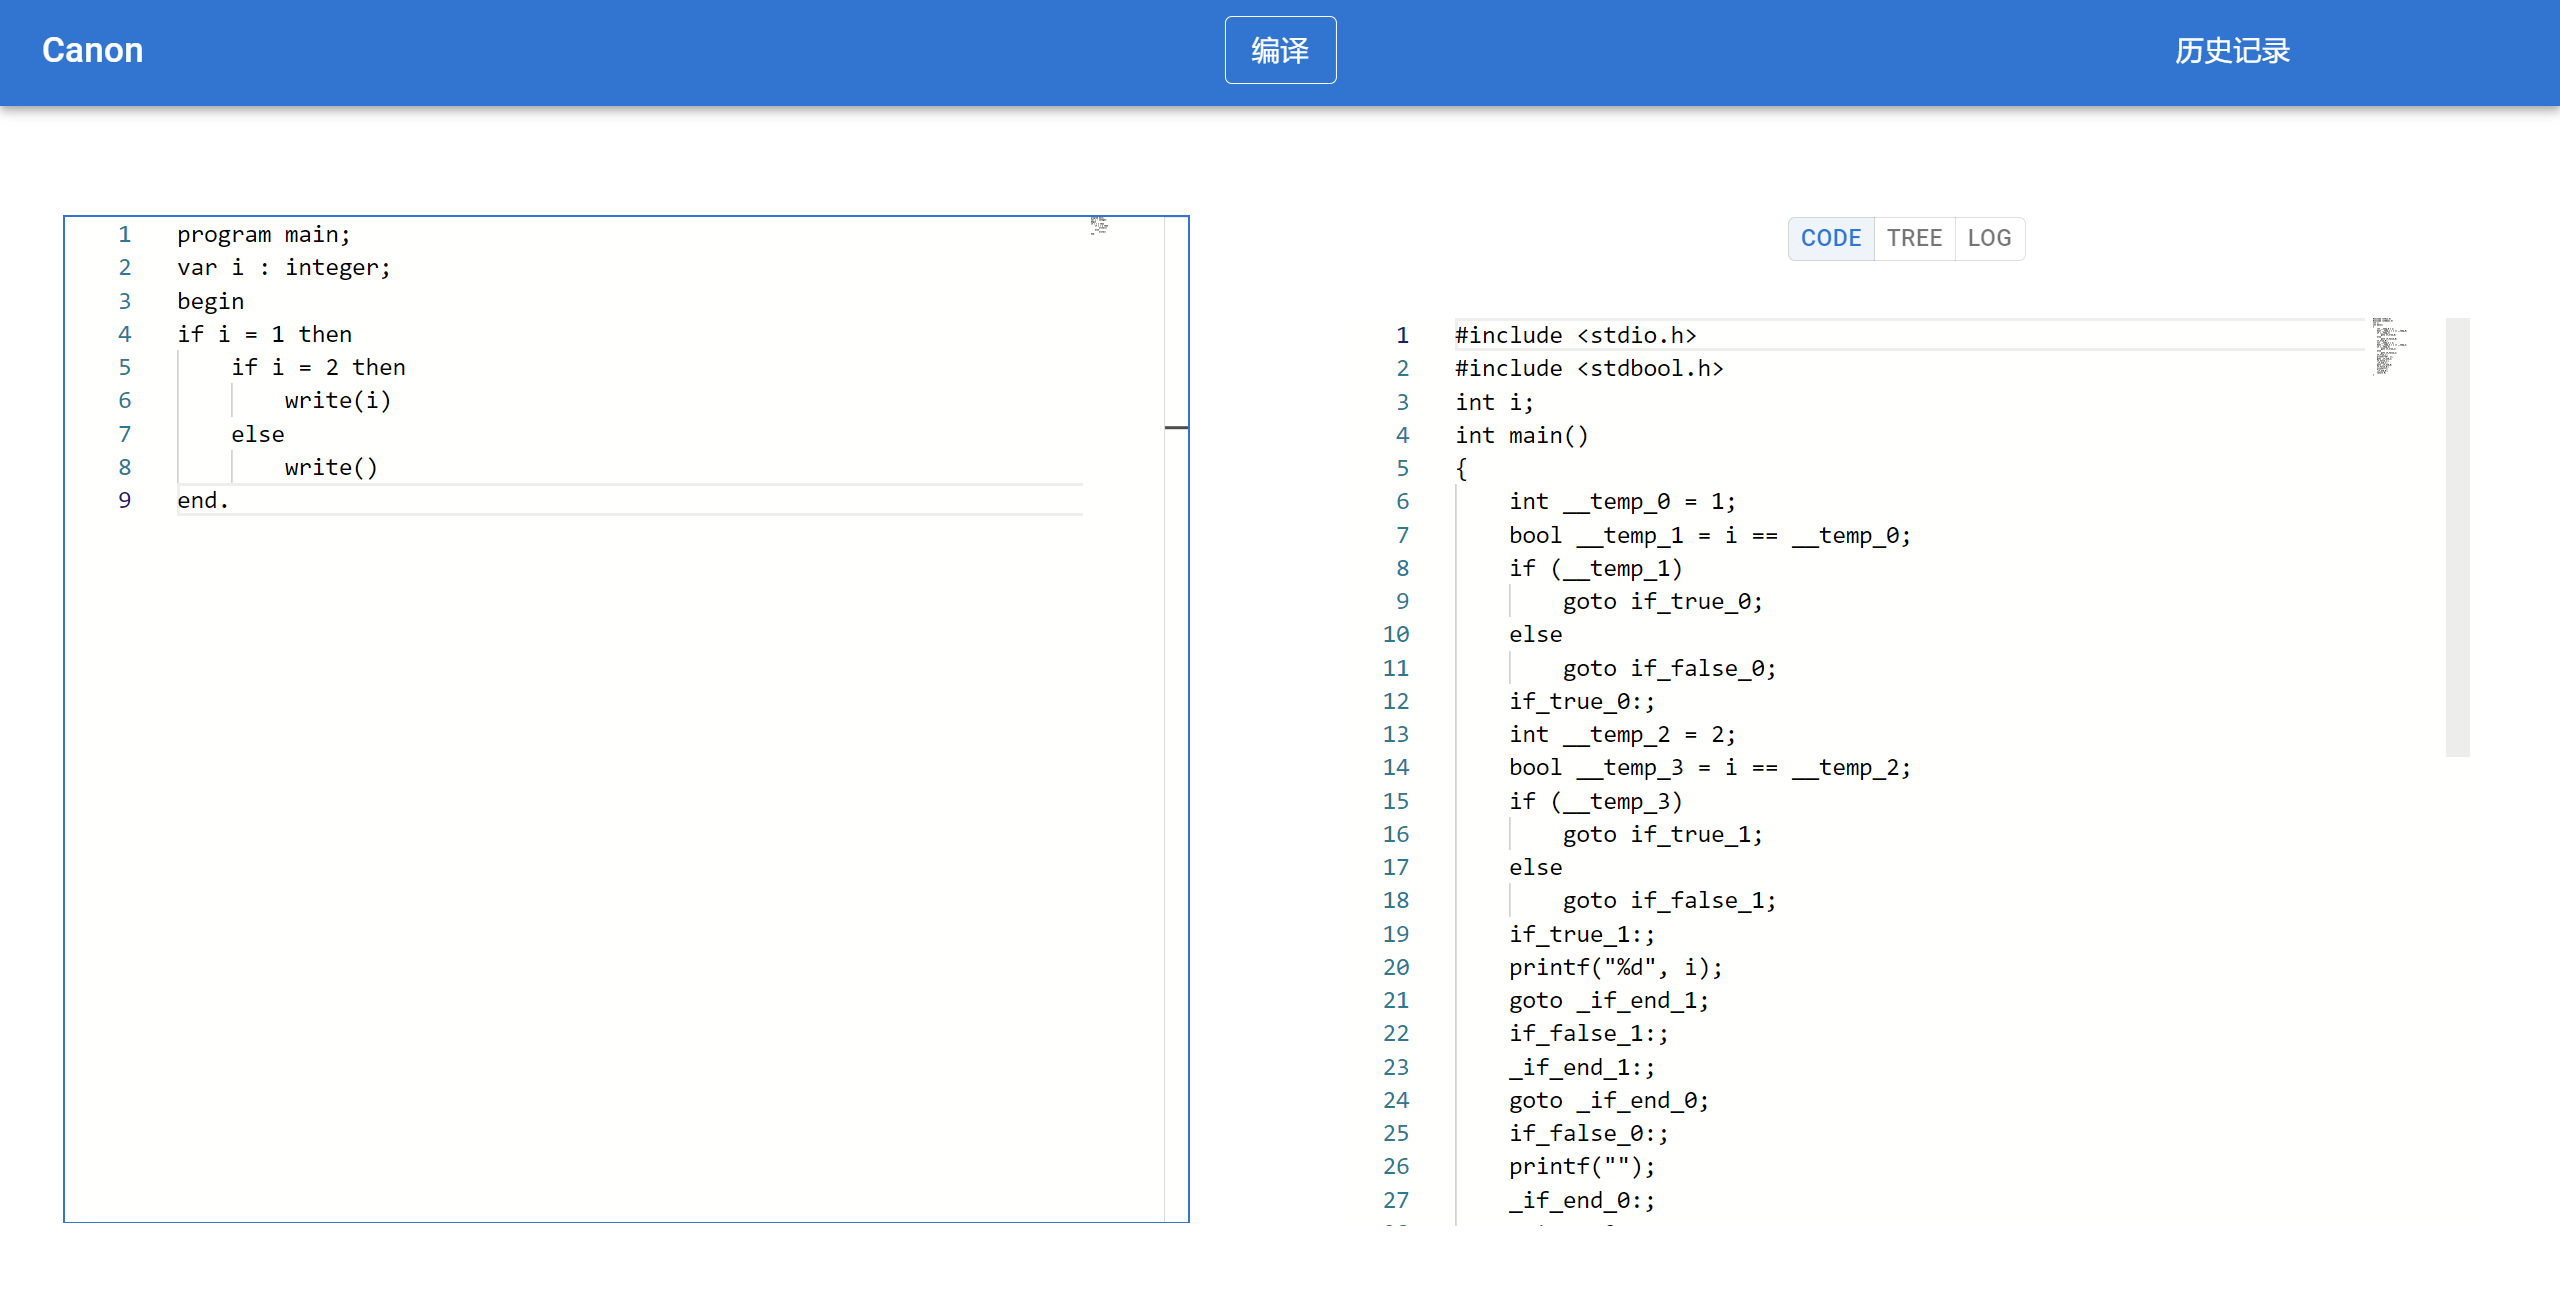
\includegraphics[width=0.9\linewidth]{assets/编译器Web在线版本.png}
    \caption{编译器Web在线版本}
    \label{fig:compiler_web_fig}
\end{figure}

Web在线版本提供了一个图形化界面,允许用户在网页上直接输入Pascal 源代码,并在线编译和查看生成的 C 代码。这为没有命令行使用经验的用户提供了便利(图\ref{fig:compiler_web_fig})。同时,图形化界面提供了Pascal源代码生成的语法树示意图(图\ref{fig:compiler_web_fig_tree}),可供用户查看并分析语法树结构。

\begin{figure}[h]
    \centering
    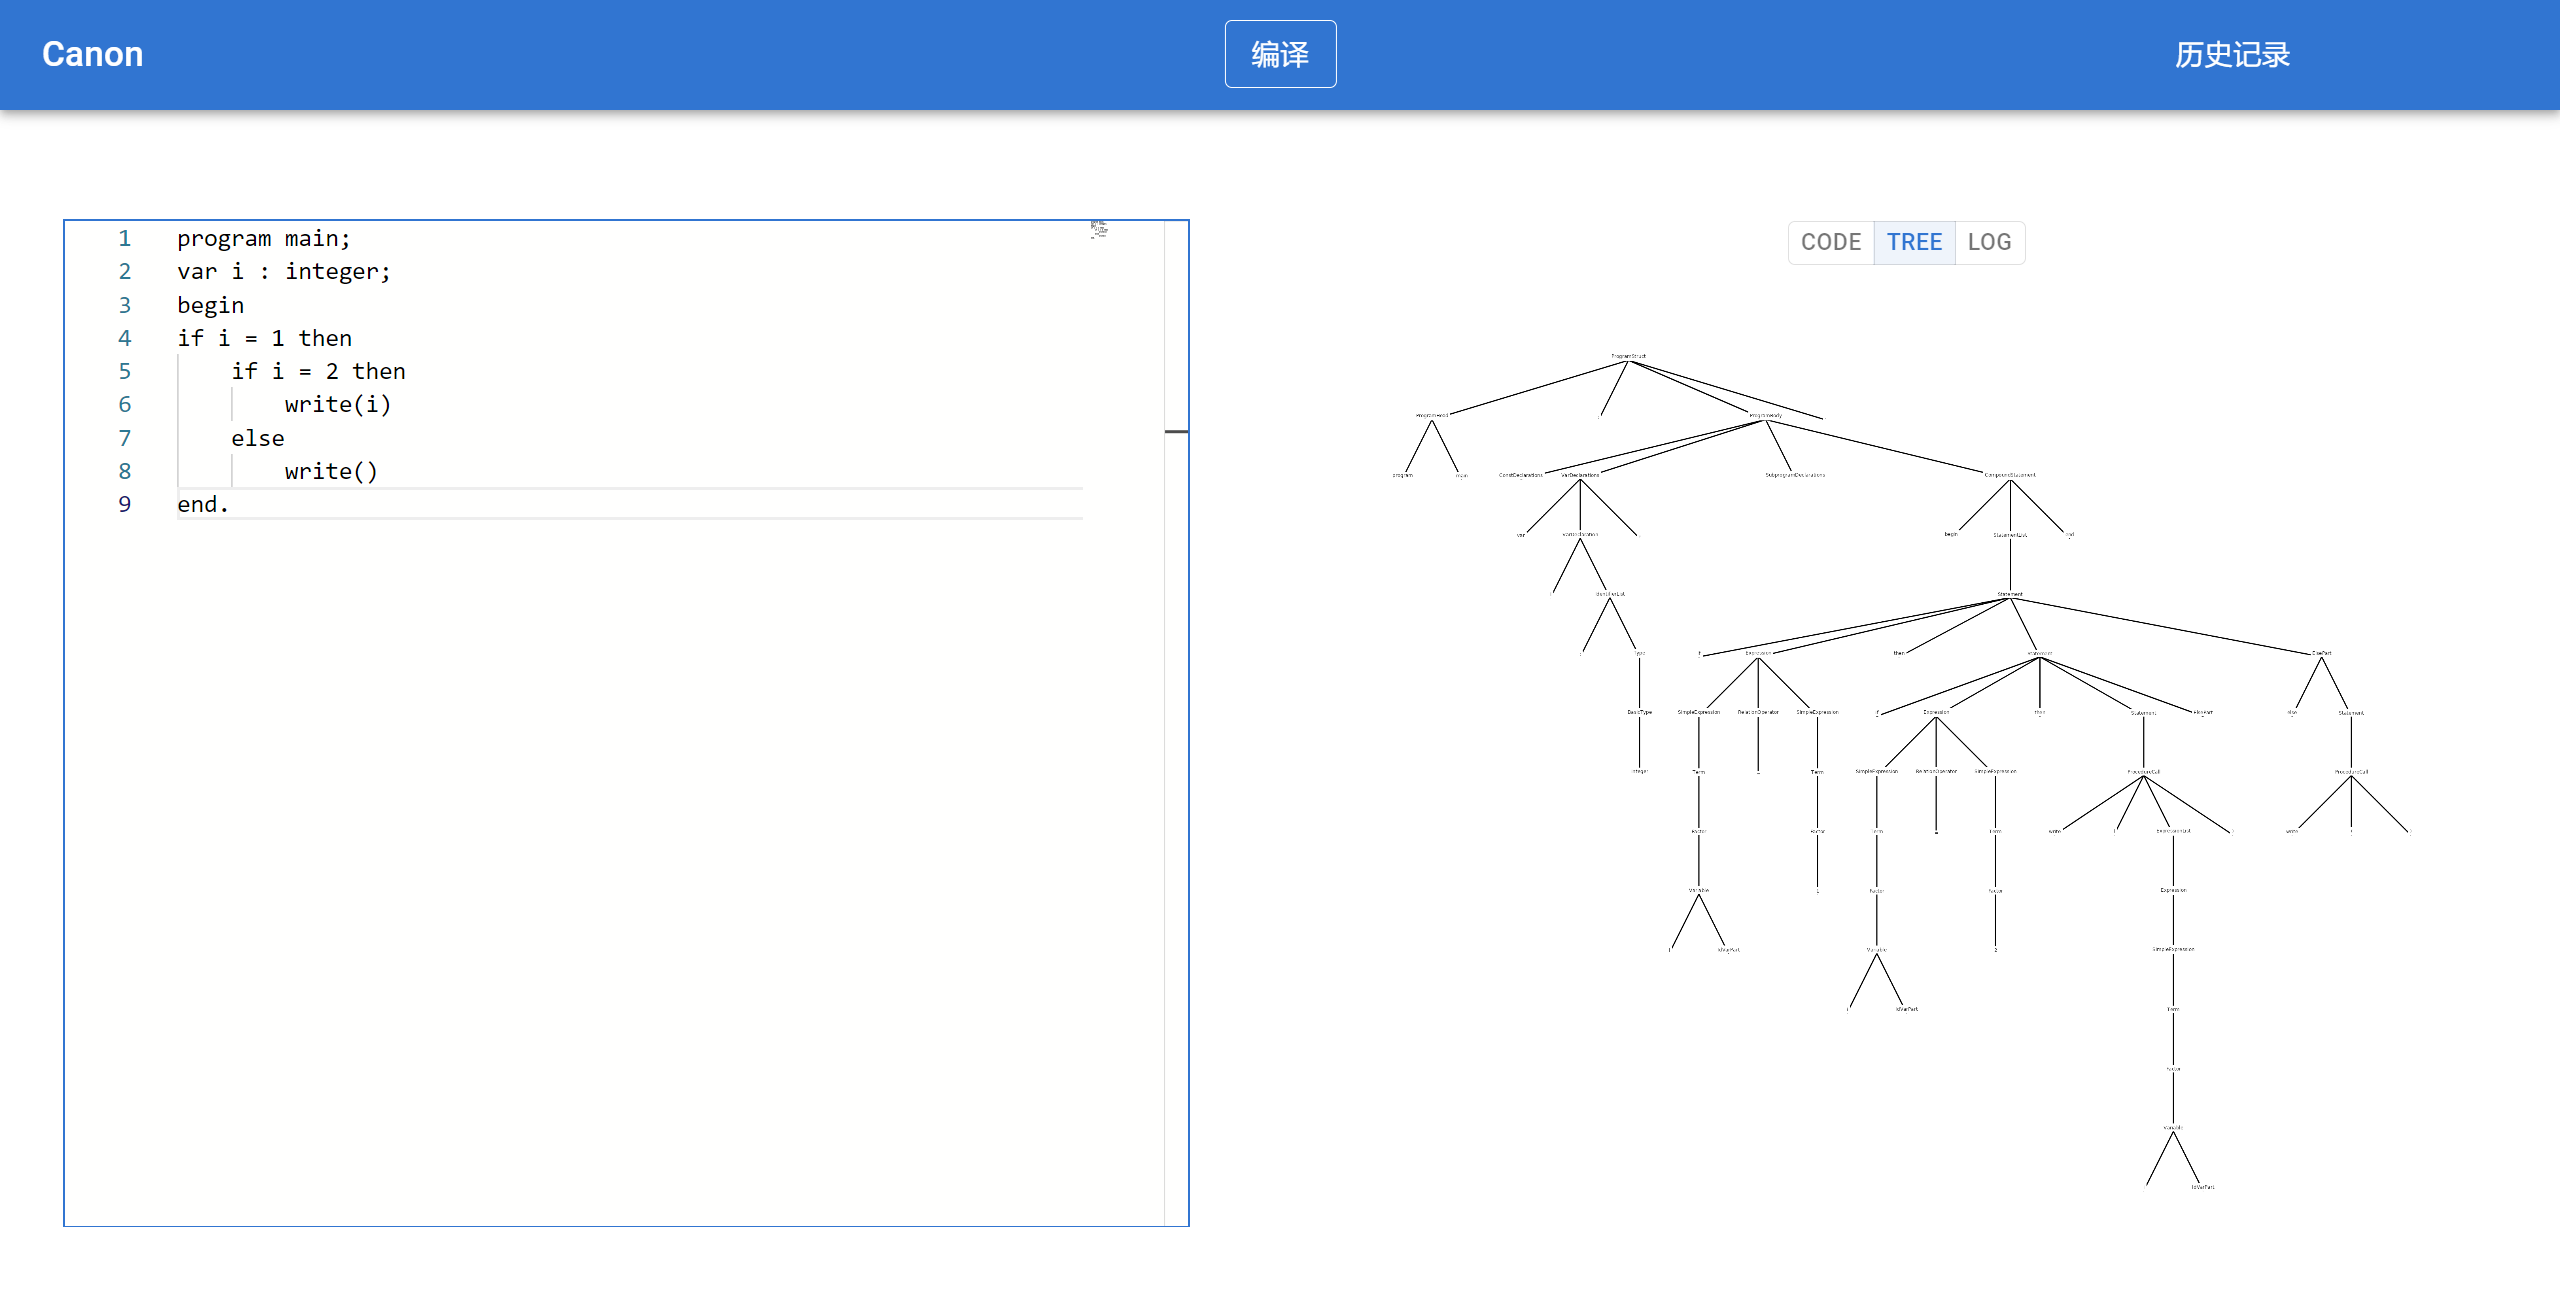
\includegraphics[width=0.9\linewidth]{assets/编译器Web在线版本_语法树.png}
    \caption{语法树渲染}
    \label{fig:compiler_web_fig_tree}
\end{figure}

Web版本的特点包括:

\begin{itemize}
    \item \textbf{代码编辑器}:集成代码编辑器,支持语法高亮,提供更好的代码编写体验。
    \item \textbf{实时编译}:用户输入代码后,可以实时编译并显示输出结果。
    \item \textbf{错误提示}:编译过程中的错误会在网页上直接显示,方便用户快速定位问题。
    \item \textbf{语法树渲染}:编译过程中,会根据输入的代码,渲染出对应的语法树。语法树上节点对应的记号类型。
    \item \textbf{历史记录}:编译器会保存成功编译的记录,并提供查看历史记录的功能。使用唯一id作为历史记录标识,实现了通过连接分享一个编译记录的功能(图\ref{fig:compiler_web_fig_history})。
\end{itemize}

\textit{注: 在实现语法树的可视化过程中,我们参考了论文\cite{goos_improving_2002}以在线性时间复杂度中绘制完整棵树。}

\begin{figure}[h]
    \centering
    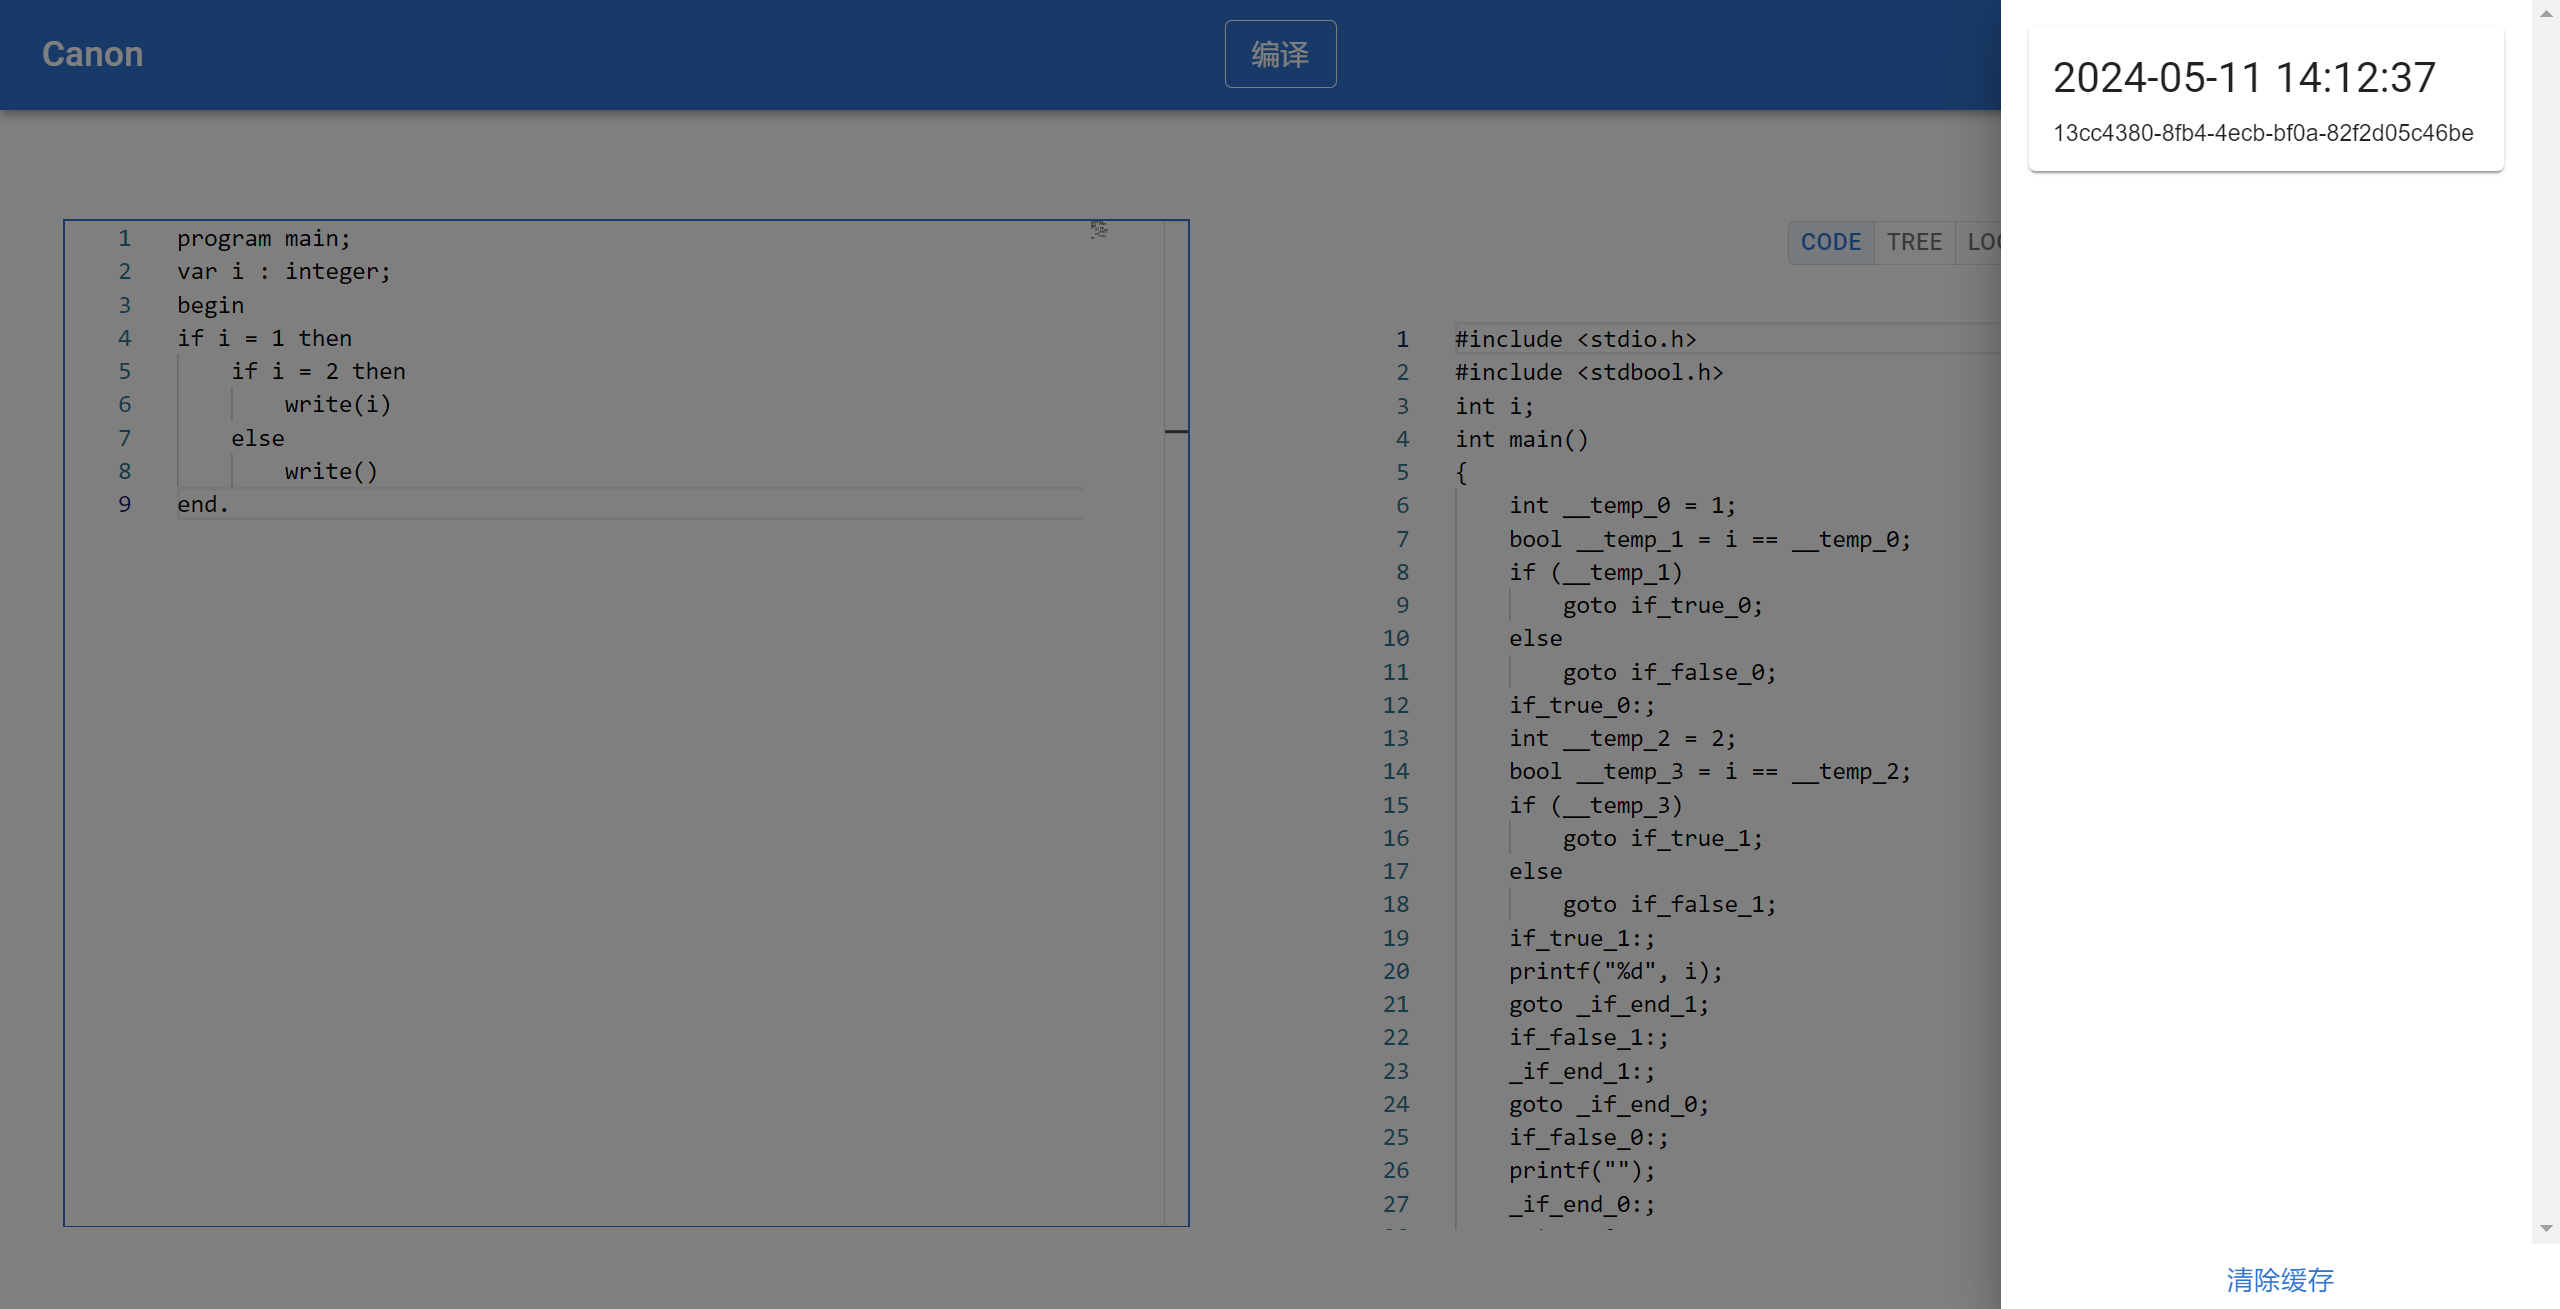
\includegraphics[width=0.9\linewidth]{assets/编译器Web在线版本_历史记录.png}
    \caption{历史记录}
    \label{fig:compiler_web_fig_history}
\end{figure}

Web在线版本的实现依赖于前后端分离的架构,前端使用React框架提供用户交互界面,后端处理编译任务。通过 AJAX 请求与后端通信,实现代码的提交和结果的获取。

总体来说,用户接口设计考虑了不同用户群体的使用习惯和需求,提供了灵活、友好的使用方式,使得用户可以更加方便地使用。

\end{document}